\documentclass[12pt]{article}

\usepackage{fullpage}
\usepackage{multicol,multirow}
\usepackage{tabularx}
\usepackage{listings}
\usepackage{pgfplots}
\usepackage[utf8]{inputenc}
\usepackage[russian]{babel}
\usepackage{pgfplots}
\usepackage{tikz}

% Оригиналный шаблон: http://k806.ru/dalabs/da-report-template-2012.tex

\begin{document}

\section*{Лабораторная работа №7\, по курсу дискрeтного анализа: Жадные алгоритмы}

Выполнил студент группы М8О-312Б-22 МАИ \textit{Юрков Евгений}.

\subsection*{Условие}

\textbf{Вариант:} 6

Заданы N объектов с ограничением на расположение вида "A должен находится перед B".
Необходимо найти такой порядок расположения объектов, что все ограничения будут выполняться.

\textbf{Формат ввода:}
На первой строке два числа, N и M, за которыми следует M строк с ограничениями вида «A B»
 ($1 \leq A, B \leq N$) определяющими относительную последовательность объектов с номерами A и B.

\textbf{Формат вывода:}
$-$1 если расположить объекты в соответствии с требованиями невозможно,
последовательность номеров объектов в противном случае.

\newpage
\subsection*{Метод решения}

Для решения задачи строился граф зависимостей элементов, то есть если элемент A стоит перед B,
то $A \rightarrow B$. Если в графе есть циклы, то задача не имеет решения, так как не существует элемента, который не зависит от остальных
и, соответственно, может стоять в начале. В процессе обхода в глубину полученного графа находился ответ, элементы, расположенные ниже
ставятся в конец, а потом элементы, которые выше, ставятся в начало.

% \newpage
\subsection*{Описание программы}

Для решения задачи была написана функция \texttt{have\_cycles}, которая проверяет граф на наличие циклов.
Основная логика содержится в функции dfs, где совершается обход графа и добавление вершин в начало списка
\texttt{answer}, представленного классом \texttt{std::list}.

%\newpage
\subsection*{Дневник отладки}

Программа получила статус "OK" с первой попытки.

\newpage
\subsection*{Тест производительности}

Написанный алгоритм имеет ту же сложность, что и обход графа в глубину, а именно $O(n + m)$
\begin{figure}
    \centering
    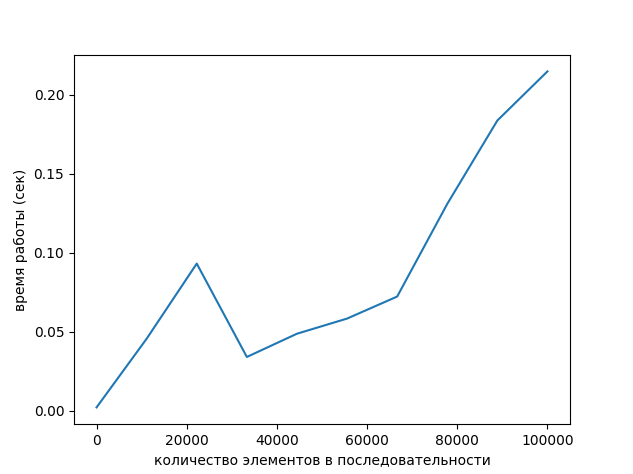
\includegraphics[width=\textwidth]{graph.png}
    \caption{График зависимости времени работы программы от длины полседовательности}
\end{figure}

% \newpage
\subsection*{Выводы}

В процессе выполнения лабораторной работы я улучшил свои навыки в решении задач, связанных с жадными алгоритмами.

\end{document}